\section{Implementation}
\label{sec:Implementation}

%%%%%%%%%%%%%%%%%%%%%%%
% 3. Implementation (describe the details of what you did, possibly divided in sections, one per major subsystems, e.g., navigation, mapping, HRI, task coordination and integration/architectures)
%%%%%%%%%%%%%%%%%%%%%%%

This section describes how the EKF with it's three basic steps has been implemented for the faced robot localization problem with a LRF. In subsection \ref{subsec:Prediction} the motion model and the observation model are discussed. The subsections \ref{subsec:Matching} and \ref{subsec:Update} deal with the matching respectively the update step. The resulting scheme of the implementation is shown in figure \ref{fig:EKF_scheme}. 

\begin{figure}[h]
\centering
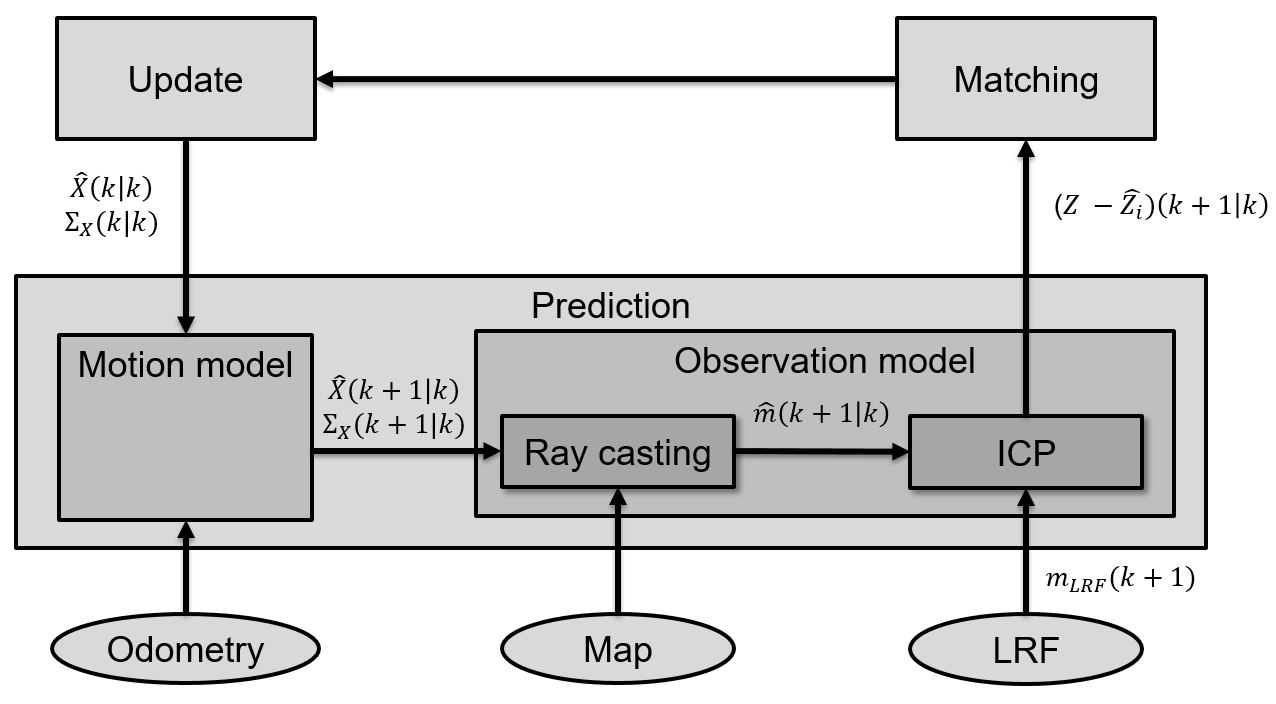
\includegraphics[width=0.45\textwidth]{figures/scheme}
      \caption{Scheme of the implemented EKF}
      \label{fig:EKF_scheme}
\end{figure}

The robot's state $X$ is defined as it's current two dimensional pose. The observation $Z$ used for the Extended Kalman filter, like explained in section \ref{subsec:Matching}, also includes variables to describe a pose. 
\begin{align}
X&=\begin{pmatrix}x_s & y_s & \theta_s \end{pmatrix}^T \label{eq:state_def} \\
Z&=\begin{pmatrix}x_{obs} & y_{obs} & \theta_{obs} \end{pmatrix}^T \label{eq:observation_def}
\end{align}

With the state and the observation being a 3 by 1 vector, the dimensions of all the variables used in the EKF are defined. Table \ref{tab:Variables_def} lists the used variables with their symbols, dimensions and a short description..
\begin{table}[h]
\centering
\begin{tabular}{>{\centering\arraybackslash}p{1.5cm} >{\centering\arraybackslash}p{1.5cm} >{\small}p{4.5cm}}%{lcc}
\toprule
Symbol & Dimension & Description \\
\midrule
$X$ & 3 x 1 & State vector - Robot pose \\
$Z$ & 3 x 1 & Observation \\
$\Sigma$ & 3 x 3 & Robot state covariance  \\
$f$ & 3 x 1 & Robot motion model function \\
$F$ & 3 x 3 & Robot motion Jacobian \\
$Q$ & 3 x 3 & Motion noise \\
$U$ & 2 x 1 & Motion input \\
$m^{i}$ & 2 x 1 & Laser beam measurement \\
$h$ & 3 x 1 & Observation model function \\
$H$ & 3 x 3 & Observation Jacobian \\
$R$ & 3 x 3 & Observation noise \\
$K$ & 3 x 3 & Kalman gain \\
\bottomrule
\end{tabular}
\caption{Variables and functions used for the EKF}
\label{tab:Variables_def}
\end{table}

\subsection{Prediction}
\label{subsec:Prediction}
The aim of the EKF prediction step is to receive the updated state and covariance and then from there on determine the predicted observation for the next time step $\widehat{Z}_i(k+1|k)$. To do so, the motion model predicts the future state in the next time step $\widehat{X}(k+1|1)$ and the corresponding covariance matrix $\Sigma_X (k+1|k)$. From there on it is possible for the observation model to obtain the predicted observation $\widehat{Z}_i(k+1|k)$. 
The motion and observation model need to be defined by the user depending on the problem and solution approach.
\subsubsection{State Prediction}
\label{subsubsec:subsubsection_Tag}
As the considered robot is a three-wheeled vehicle that drives in a planar two dimensional environment, a motion model can be developed for specifically for this case. The Pioneer 3DX is steered by giving different speed commands to the left and right wheel. Therefore, the motion input vector is defined as in \eqref{eq:input}.
 
\begin{equation}
U=\begin{pmatrix}\omega_{Right} & \omega_{Left} \end{pmatrix}^T \label{eq:input}
\end{equation}
\noindent \begin{tabularx}{\textwidth}{@{}XXX@{}}
\begin{equation} 
\beta=\frac{\omega_{Right}-\omega_{Left}}{d} \label{eq:beta}
\end{equation} &
\begin{equation}
R=\frac{\omega_{Left}}{\beta} \label{eq:R}
\end{equation}
\end{tabularx}
With the help of $d$, the distance between the robot's driven wheels, and the defined parameters $R$ and $\beta$ in \eqref{eq:beta} respectively \eqref{eq:R}, it is possible to formulate the motion model in equation \eqref{eq:MotionModel}.
\begin{align}
&X(k+1|k)=f(X(k),~U(k)) \nonumber\\ &= \begin{pmatrix} x_s(k) + (R+\frac{d}{2})(sin(\theta+ \beta)-sin(\theta)) \\ y_s(k) + (R+{{d}\over{2}})(-cos(\theta+ \beta)+cos(\theta)) \\ \theta_s(k) + \beta\end{pmatrix}
\label{eq:MotionModel}
\end{align}

\subsubsection{Observation Prediction}
\label{subsubsec:subsubsection_Tag}
Subsubsection text here.

\subsection{Matching}
\label{subsec:Matching}
Maybe add the anti-kidnapping stuff to the scheme picture.

\subsection{Update}
\label{subsec:Update}
Subsection text here.

%\subsubsection{Subsubsection Heading Here}
%\label{subsubsec:subsubsection_Tag}
%Subsubsection text here.
